\begin{tikzpicture}
    \node[anchor=south west,inner sep=0] (image) at (4.0,0) {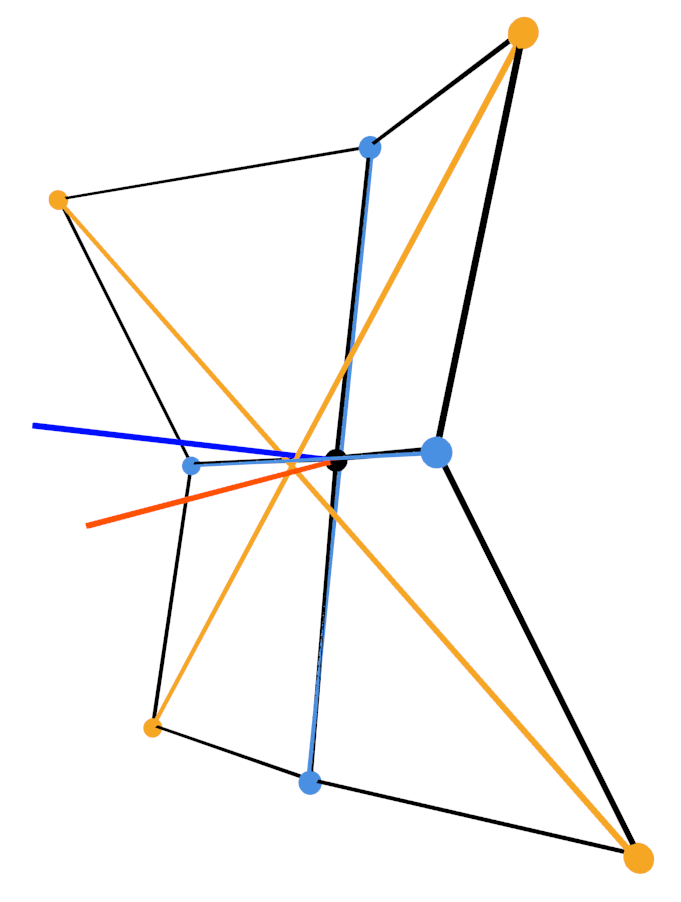
\includegraphics[width=0.6\textwidth]{chapter04/img/flexion-model-2-clipped.png}};
    \node at (4.4, 5.1) {$\mathbf{P_{i-1,j-1}}$};
    \node at (6.2, 5.5) {$\mathbf{P_{i,j-1}}$};
    \node at (8.5, 5.8) {$\mathbf{P_{i+1,j-1}}$};

    \node at (4.7, 2.9) {\scalebox{0.9}{$\mathbf{P_{i-1,j}}$}};
    \node at (6.2, 2.5) {$\mathbf{P_{i,j}}$};
    \node at (7.7, 3.0) {$\mathbf{P_{i+1,j}}$};

    \node at (5.0, 0.9) {$\mathbf{P_{i-1,j+1}}$};
    \node at (6.3, 0.4) {$\mathbf{P_{i,j+1}}$};
    \node at (9.2, 0.3) {$\mathbf{P_{i+1,j+1}}$};

    \node [plotdarkblue] at (4.6, 3.5) {$\vec{n_1}$};
    \node [plotdarkorange] at (4.8, 2.3) {$\vec{n_2}$};
\end{tikzpicture}
